\documentclass[10pt,twocolumn,letterpaper]{article}

% --- Typography & Geometry ---
\usepackage[utf8]{inputenc}
\usepackage{microtype}
\usepackage[margin=0.75in,top=0.85in,bottom=0.85in]{geometry}

% --- Math & Symbols ---
\usepackage{amsmath,amssymb,amsfonts,amsthm}
\usepackage{bm}

% --- Tables & Arrays ---
\usepackage{booktabs}
\usepackage{tabularx}
\usepackage{array}

% --- Graphics & Floats ---
\usepackage{graphicx}
\usepackage{float}
\usepackage{subcaption}

% --- Code Listings ---
\usepackage{xcolor}
\usepackage{listings}

\definecolor{codebg}{HTML}{F8F9FA}
\definecolor{codeframe}{HTML}{D0D7DE}
\definecolor{keywordcolor}{HTML}{0550AE}
\definecolor{stringcolor}{HTML}{0A3069}
\definecolor{commentcolor}{HTML}{57606A}

\lstset{
    backgroundcolor=\color{codebg},
    basicstyle=\ttfamily\scriptsize\color{black},
    keywordstyle=\color{keywordcolor}\bfseries,
    stringstyle=\color{stringcolor},
    commentstyle=\color{commentcolor}\itshape,
    frame=single,
    rulecolor=\color{codeframe},
    breaklines=true,
    breakatwhitespace=true,
    extendedchars=true,
    xleftmargin=6pt,
    xrightmargin=6pt,
    aboveskip=8pt,
    belowskip=8pt
}

% --- Hyperlinks ---
\usepackage{hyperref}
\hypersetup{
    colorlinks=true,
    linkcolor=blue!70!black,
    citecolor=blue!70!black,
    urlcolor=blue!70!black
}

% --- Input Title & Authors ---
\section{BAM-UMoE: Unified Mixture of Experts Attention with Step-0 Representation Preservation}

\textbf{Authors:}
\begin{itemize}
\item {{AUTHOR\_1\_NAME}}  -- {{AUTHOR\_1\_EMAIL}}
\end{itemize}
\begin{itemize}
\item {{AUTHOR\_2\_NAME}}  -- {{AUTHOR\_2\_EMAIL}}
\end{itemize}

\textbf{Affiliations:}
\begin{itemize}
\item   {{UNIVERSITY\_1}}, {{DEPARTMENT\_1}}
\end{itemize}
\begin{itemize}
\item   {{UNIVERSITY\_2}}, {{DEPARTMENT\_2}}
\end{itemize}

\textbf{Preprint date:} {{DATE}}
\textbf{Version:} v{{VERSION}}
\textbf{Code:} https://github.com/{{ORG}}/SVD\_Project/tree/main/framework/attentions/bam\_umoe.py
\textbf{License:} {{LICENSE}}



\subsection{Abstract}

Mixture of Experts (MoE) layers increase transformer capacity without 
proportional compute increases, but applying MoE to **attention value 
refinement** post-hoc is non-trivial: random initialization perturbs the 
pretrained representation, destabilizing recovery. We introduce \textbf{BAM-UMoE} 
(\textbf{B}idirectional \textbf{A}ttention \textbf{M}odulation with \textbf{U}nified \textbf{M}ixture 
\textbf{of E}xperts), which appends a top-2 MoE branch to the value pathway of 
each attention block with a \textbf{three-part step-0 preservation mechanism}:

1. \textbf{Zero-initialized final expert layers.} Every expert's output projection 
   starts at exactly zero, so the MoE branch contributes nothing at step 0.
2. \textbf{Negative gating bias.} A learnable gate with bias initialized to $-3.0$ 
   produces $\sigma(-3) \approx 0.047$, gently ramping up MoE contribution.
3. \textbf{Frozen base attention.} The original $W_Q, W_K, W_V, W_O$ projections 
   are copied exactly and frozen; only LoRA adapters and the MoE branch train.

The combination guarantees that **the initial forward pass is mathematically 
identical to the pretrained model**, allowing MoE capacity to be added without 
catastrophic drift.

BAM-UMoE supports flat (DistilBERT), nested (RoBERTa/BERT), causal (GPT-2), 
and GQA+RoPE (Qwen/LLaMA) architectures without modification. It additionally 
supports \textbf{cross-attention} for encoder-decoder models, and handles Conv1D 
fusions, nested encoders, and padding-aware masking natively.

\textbf{Important disclosure.} BAM-UMoE is \textbf{not} a compression method. Adding 
8 experts per layer increases parameter count substantially (see Table 7.2); 
we report all costs transparently. The method's value lies in **capacity 
expansion** rather than size reduction.

\textbf{Keywords:} mixture of experts, attention refinement, step-0 preservation, 
LoRA, multi-architecture



\subsection{Lay Summary}

Mixture of Experts (MoE) is a technique where multiple small "expert" networks 
process the same input, and a router decides which experts to use for each 
token. This increases model capacity without proportionally increasing 
compute. Applying MoE to a \textbf{pretrained} transformer is hard: random 
initialization perturbs the model and destroys its pretrained knowledge. 
BAM-UMoE solves this by carefully initializing the MoE branch so that at 
training step 0, the model behaves exactly like the pretrained model. Then, 
during fine-tuning, the MoE branch gradually "wakes up" and learns to add 
value. The trade-off is a substantial increase in model size -- this is a 
capacity expansion method, not a compression method.



\subsection{Table of Contents}

1. [Introduction](01\_intro.md)
2. [Related Work](02\_related.md)
3. [Background](03\_background.md)
4. [Method](04\_method.md)
5. [Architecture Integration](05\_architecture.md)
6. [Experimental Setup](06\_setup.md)
7. [Results](07\_results.md)
8. [Analysis](08\_analysis.md)
9. [Discussion](09\_discussion.md)
10. [Limitations](10\_limitations.md)
11. [Conclusion](11\_conclusion.md)
12. [Reproducibility](12\_reproducibility.md)
13. [References](13\_references.md)

\textbf{Appendices:}
\begin{itemize}
\item [A. Mathematical Derivations](A\_math.md)
\end{itemize}
\begin{itemize}
\item [B. Implementation Details](B\_implementation.md)
\end{itemize}
\begin{itemize}
\item [C. Full Experimental Data](C\_data.md)
\end{itemize}
\begin{itemize}
\item [D. Negative Results](D\_negative\_results.md)
\end{itemize}
\begin{itemize}
\item [E. Ethical Considerations](E\_ethics.md)
\end{itemize}

\begin{document}

\maketitle

% --- Abstract & Keywords Block ---
\begin{abstract}
Mixture of Experts (MoE) layers increase transformer capacity without 
proportional compute increases, but applying MoE to **attention value 
refinement** post-hoc is non-trivial: random initialization perturbs the 
pretrained representation, destabilizing recovery. We introduce **BAM-UMoE** 
(**B**idirectional **A**ttention **M**odulation with **U**nified **M**ixture 
**of E**xperts), which appends a top-2 MoE branch to the value pathway of 
each attention block with a **three-part step-0 preservation mechanism**:

1. **Zero-initialized final expert layers.** Every expert's output projection 
   starts at exactly zero, so the MoE branch contributes nothing at step 0.
2. **Negative gating bias.** A learnable gate with bias initialized to $-3.0$ 
   produces $\sigma(-3) \approx 0.047$, gently ramping up MoE contribution.
3. **Frozen base attention.** The original $W_Q, W_K, W_V, W_O$ projections 
   are copied exactly and frozen; only LoRA adapters and the MoE branch train.

The combination guarantees that **the initial forward pass is mathematically 
identical to the pretrained model**, allowing MoE capacity to be added without 
catastrophic drift.

BAM-UMoE supports flat (DistilBERT), nested (RoBERTa/BERT), causal (GPT-2), 
and GQA+RoPE (Qwen/LLaMA) architectures without modification. It additionally 
supports **cross-attention** for encoder-decoder models, and handles Conv1D 
fusions, nested encoders, and padding-aware masking natively.

**Important disclosure.** BAM-UMoE is **not** a compression method. Adding 
8 experts per layer increases parameter count substantially (see Table 7.2); 
we report all costs transparently. The method's value lies in **capacity 
expansion** rather than size reduction.

**Keywords:** mixture of experts, attention refinement, step-0 preservation, 
LoRA, multi-architecture

---

\vspace{0.5em}
\noindent\textbf{Keywords:} mixture of experts, attention refinement, step-0 preservation,
\end{abstract}

\vspace{1em}

% --- Paper Body ---
\section{1. Introduction}

\subsection{1.1 Motivation}

Mixture of Experts (MoE) has emerged as a powerful technique for scaling 
transformer capacity without proportional compute (Shazeer et al., 2017; 
Fedus et al., 2022; Lepikhin et al., 2021). In a standard MoE, a router 
selects top-$k$ experts per token, and only the selected experts run forward 
passes. This gives the model more "knowledge slots" while keeping FLOPs 
roughly constant.

\textbf{The pretrained-model problem.} Most MoE methods are applied during 
pretraining: experts and routers are initialized randomly and trained 
end-to-end on a large corpus. Applying MoE \textbf{post hoc} to an already 
pretrained transformer is more delicate. Random initialization of the MoE 
branch perturbs the pretrained representation, causing catastrophic 
forgetting and necessitating extensive recovery training.

\textbf{A three-part solution.} BAM-UMoE solves this with:

1. \textbf{Zero-initialized experts.} Every expert's final output projection 
   starts at exactly zero. The MoE branch therefore contributes nothing 
   to the forward pass at step 0.

2. \textbf{Negative gating bias.} A learnable gate with initial bias $-3.0$ 
   produces $\sigma(-3) \approx 0.047$, meaning the MoE branch is attenuated 
   by ~95\% at start. As training progresses, the gate learns to open.

3. \textbf{Frozen base attention.} The pretrained $W_Q, W_K, W_V, W_O$ are copied 
   exactly and frozen. LoRA adapters provide trainable capacity, and the MoE 
   branch provides additional routing capacity.

Together, these ensure that **step 0 is mathematically identical to the 
pretrained model**.

\subsection{1.2 Problem Statement}

Given a pretrained attention module with projections 
$W_Q, W_K, W_V, W_O \in \mathbb{R}^{d \times d}$ and a target task, we seek 
an augmented attention module $\mathcal{A}'$ that:

1. \textbf{Preserves step-0 behavior.} $\mathcal{A}'(X) = \mathcal{A}(X)$ for 
   all inputs $X$ at initialization.
2. \textbf{Adds capacity.} The augmented module has more trainable parameters 
   than the original, but not more activation FLOPs.
3. \textbf{Supports recovery fine-tuning.} Only a small fraction of parameters 
   is trainable, minimizing catastrophic forgetting.
4. \textbf{Works across architectures.} Flat (DistilBERT), nested (RoBERTa), 
   causal (GPT-2), and GQA+RoPE (Qwen/LLaMA).

\textbf{Note.} This is \textbf{not} a compression method. Parameter count increases 
substantially; the goal is capacity expansion with stable recovery.

\subsection{1.3 Our Approach}

BAM-UMoE augments the \textbf{value pathway} of attention with a top-$k$ MoE 
branch:

\[
V' = V_{\text{base}} + \alpha \cdot \text{MoE}(X)
\tag{1.1}
\]

where $X$ is the input hidden states, $V_\text{base} = X W_V^\top$ is the 
frozen base value projection, and MoE$(X)$ is a top-$k$ expert mixture 
producing a refinement signal of the same shape. The coefficient $\alpha = 0.1$ 
scales the MoE contribution conservatively.

\textbf{Key property.} At initialization, MoE$(X) = 0$ because every expert's 
output projection is zero. Step 0 is exact.

\subsection{1.4 Contributions}

\begin{itemize}
\item \textbf{A three-part step-0 preservation mechanism.} Zero-init + negative
\end{itemize}
  gating bias + frozen base. Section 4.3.
\begin{itemize}
\item \textbf{A top-2 MoE attention refinement.} A vectorized expert mixture applied
\end{itemize}
  to the value pathway with an auxiliary load-balancing loss. Section 4.2.
\begin{itemize}
\item \textbf{Broad architecture support.} Multi-architecture weight extraction plus
\end{itemize}
  nested encoder detection, GQA, RoPE with partial dims, and cross-attention. 
  Section 5.
\begin{itemize}
\item \textbf{Honest disclosure.} We clearly state that BAM-UMoE \textbf{increases}
\end{itemize}
  parameter count. Section 7.2.
\begin{itemize}
\item \textbf{Full reproducibility.} Code, checkpoints, and evaluation scripts released
\end{itemize}
  under {{LICENSE}}.

\subsection{1.5 Paper Organization}

Section 2 reviews related work. Section 3 provides background on MoE, LoRA, 
and step-0 preservation. Section 4 presents the method. Section 5 describes 
architecture integration. Section 6 details the experimental setup. Section 7 
reports results. Section 8 analyzes the step-0 property and ablation 
contributions. Section 9 discusses usage. Section 10 lists limitations. 
Section 11 concludes.



\subsection{Notation}

\section{Related Work}

\subsection{Mixture of Experts}

\textbf{Switch Transformer.} Fedus et al. (2022) simplify MoE to top-1 routing, 
reducing communication overhead while maintaining capacity. BAM-UMoE uses 
top-2 routing, which has been shown to give better quality per FLOP.

\textbf{GShard.} Lepikhin et al. (2021) introduce top-2 gating with auxiliary 
load-balancing loss. BAM-UMoE uses the same formulation for its MoE branch.

\textbf{Expert Choice.} Zhou et al. (2022) reverse the routing direction: experts 
choose tokens instead of tokens choosing experts. Orthogonal to our approach.

\textbf{Soft MoE.} Puigcerver et al. (2023) use soft routing without discrete 
top-k. BAM-UMoE uses hard top-2 for simplicity.

\subsection{Post-Hoc MoE}

\textbf{MoEfication.} Zhang et al. (2022) split pretrained FFN layers into 
multiple experts without retraining. BAM-UMoE is orthogonal -- it adds new 
capacity rather than partitioning existing capacity.

\textbf{Sparse Upcycling.} Komatsuzaki et al. (2023) initialize MoE from a dense 
model by duplicating FFN weights. BAM-UMoE does not duplicate; it adds 
a zero-initialized MoE branch.

\textbf{Lifelong MoE.} Chen et al. (2023) adapt MoE to new tasks while preserving 
old ones. Different motivation.

\subsection{Parameter-Efficient Fine-Tuning}

\textbf{LoRA.} Hu et al. (2021) parameterize a weight update with a low-rank 
product $BA$, $B = 0$ at initialization. BAM-UMoE uses LoRA for base 
attention adaptation alongside the MoE branch.

\textbf{AdaLoRA.} Zhang et al. (2023) allocate LoRA rank adaptively. Orthogonal.

\textbf{PiSSA.} Meng et al. (2024) initialize LoRA from principal components. 
Compatible with BAM-UMoE.

\subsection{Attention Augmentation}

\textbf{Attention Refinement.} Many works augment attention with additional 
branches. BAM-UMoE's specific contribution is applying \textbf{MoE} to the 
value pathway.

\textbf{Gated Attention.} Gating mechanisms in attention have been studied 
(Parisotto et al., 2020; Bapna et al., 2021). BAM-UMoE uses gating to 
control the MoE contribution's ramp-up.

\subsection{Position of Our Work}

\begin{table}[H]
\centering
\small
\begin{tabular}{lll}
\toprule
\textbf{Feature} & \textbf{Prior MoE} & \textbf{BAM-UMoE} \\
\midrule
Application & Pretraining & Post-hoc \\
Step-0 preservation & Not typically & \textbf{Explicit} \\
Base weights & Trained & Frozen \\
Target & FFN capacity & \textbf{Value pathway} \\
LoRA integration & Rare & Yes \\
\bottomrule
\end{tabular}
\end{table}

BAM-UMoE is unique in explicitly targeting the \textbf{value pathway} with MoE 
and providing a \textbf{three-part step-0 preservation} mechanism.
\begin{lstlisting}

---
\end{lstlisting}
\section{Background}

\subsection{Multi-Head Attention}

For input $X \in \mathbb{R}^{B \times L \times d}$, standard attention:

\[
Q = X W_Q^\top, \quad K = X W_K^\top, \quad V = X W_V^\top
\]

\[
\text{Attn}(X) = \text{softmax}\!\left(\frac{Q K^\top}{\sqrt{d_h}}\right) V
\]

\subsection{Mixture of Experts}

An MoE layer replaces a single FFN with $E$ expert FFNs and a router:

\[
\text{MoE}(X) = \sum_{i \in \text{top-}k} g_i \cdot \text{Expert}_i(X)
\]

where $g_i$ is the router weight after softmax, and top-$k$ selects the 
$k$ highest-weighted experts. Only those experts run forward.

\textbf{Load balancing loss.} To prevent router collapse:

\[
\mathcal{L}_\text{aux} = E \cdot \sum_{e=1}^{E} f_e \cdot P_e
\]

where $f_e$ is the fraction of tokens routed to expert $e$ and $P_e$ is the 
mean router probability for expert $e$.

\subsection{The Step-0 Preservation Problem}

Adding a randomly initialized branch to a pretrained model perturbs its 
output at step 0:

\[
\mathcal{A}'(X) = \mathcal{A}(X) + \Delta(X)
\]

with $\Delta(X) \neq 0$ in general. For catastrophic forgetting this is 
harmful. BAM-UMoE enforces $\Delta(X) = 0$ at initialization via three 
mechanisms:

\begin{enumerate}
\item \textbf{Zero-init final layer.} Every expert's last linear layer is zero.
\item \textbf{Negative gating bias.} The gate outputs $\sigma(-3) \approx 0.047$.
\item \textbf{Frozen base.} Base attention weights are exact copies.

\end{enumerate}
\subsection{LoRA}

LoRA (Hu et al., 2021):

\[
\Delta W = \frac{\alpha}{r_L} B A, \quad B = 0 \text{ at init}
\]

with $A \in \mathbb{R}^{r_L \times d}$, $B \in \mathbb{R}^{d \times r_L}$.

\subsection{Grouped-Query Attention}

GQA uses $H_{kv} < H$ KV heads, repeated to match query heads. BAM-UMoE 
preserves GQA structure.

\subsection{Rotary Position Embeddings}

RoPE rotates Q, K by position-dependent angles. BAM-UMoE supports **partial 
RoPE** (Qwen3.5 with rotary\_dim < head\_dim) by rotating the first 
\texttt{rotary\_dim} coordinates.

\subsection{Notation Summary}

\begin{lstlisting}

---
\end{lstlisting}
\section{4. Method}

\subsection{4.1 Overview}

BAM-UMoE augments attention with an MoE refinement of the value pathway. 
The forward pass:

1. \textbf{Standard QKV projections} with frozen base weights ( 4.2).
2. \textbf{MoE value refinement} applied additively to V ( 4.3).
3. \textbf{Gated scaling} for controlled ramp-up ( 4.4).
4. \textbf{Output projection} with nested bypass ( 4.5).

\textbf{Figure 4.1} shows the architecture.

\begin{lstlisting}
    +------------------------------------------+
    |  Input X                                  |
    +------------------+-----------------------+
                       |
        +--------------+--------------+
        |              |              |
                                       
    +-------+      +-------+      +-------+
    | Q     |      | K     |      | V     |   $\leftarrow$ frozen base
    | proj  |      | proj  |      | proj  |   + LoRA
    +---+---+      +---+---+      +---+---+
        |              |              |
        |              |               
        |              |      +--------------+
        |              |      |  MoE Branch  |
        |              |      |  (8 experts, |
        |              |      |   top-2)     |
        |              |      +------+-------+
        |              |             |
        |              |                $\times$ 0.1 $\times$ $\sigma$(gate)
        |              |        +---------+
        |              |        | Add     |
        |              |        | to V    |
        |              |        +----+----+
        |              |             |
        +--------------+-------------+
                       |
                        
              +----------------+
              |  Attention     |
              |  (softmax)     |
              +--------+-------+
                       |
                        
              +----------------+
              | Output proj    |
              +--------+-------+
                       |
                        
                      Y
\end{lstlisting}

\subsection{4.2 Phase 1: Base Attention}

For each projection $P \in \{Q, K, V, O\}$, we use a \texttt{LoRALinear} module:

\[
\text{Proj}_P(X) = X W_P^\top + (X A_P^\top) B_P^\top \cdot s + b_P
\tag{4.1}
\]

where $W_P$ is the frozen base, $(A_P, B_P)$ are LoRA factors, and 
$s = \alpha/r_L$ is the LoRA scaling.

Base weights are copied exactly from the pretrained attention via 
\texttt{copy\\_weights} (see Section 5).

\subsection{4.3 Phase 2: MoE Value Refinement}

\subsubsection{4.3.1 MoE Architecture}

The MoE branch produces a refinement signal of shape 
$(B, L, H \cdot d_h)$:

\[
\text{MoE}(X) = \text{TopK-Gate}(X) \cdot \text{Experts}(X)
\tag{4.2}
\]

Concretely:

\[
\begin{aligned}
X_\text{norm} &= \text{LayerNorm}(X) \\
\logits &= \text{Router}(X_\text{norm}) \in \mathbb{R}^{B \times L \times E} \\
(\text{topk\_vals}, \text{topk\_idx}) &= \text{topk}(\logits, k) \\
\text{scores} &= \text{softmax}(\text{topk\_vals}) \\
E_\text{out} &= \text{stack}([\text{Expert}_e(X) \text{ for } e \in [E]]) \\
\text{MoE}(X) &= \sum_{j=1}^{k} \text{scores}_j \cdot E_\text{out}[\text{topk\_idx}_j]
\end{aligned}
\tag{4.3}
\]

\subsubsection{4.3.2 Expert Architecture}

Each expert is a 2-layer MLP:

\[
\text{Expert}_e(X) = W_2^{(e)} \cdot \text{GELU}(W_1^{(e)} X + b_1^{(e)}) + b_2^{(e)}
\tag{4.4}
\]

with $W_1^{(e)} \in \mathbb{R}^{(2d) \times d}$ and 
$W_2^{(e)} \in \mathbb{R}^{d \times (2d)}$.

\subsubsection{4.3.3 Step-0 Zero Initialization}

\textbf{Critical.} We initialize:

\[
W_2^{(e)} = 0, \quad b_2^{(e)} = 0 \quad \forall e
\tag{4.5}
\]

This ensures $\text{Expert}_e(X) = 0$ for all inputs, so 
$\text{MoE}(X) = 0$ at step 0.

\subsubsection{4.3.4 Auxiliary Load Balancing Loss}

We add the Switch/GShard load-balancing loss:

\[
\mathcal{L}_\text{aux} = E \cdot \sum_{e=1}^{E} f_e \cdot P_e
\tag{4.6}
\]

where $f_e$ is the fraction of tokens routed to expert $e$ and $P_e$ is 
the mean router probability. This is added to the task loss with weight 
$\lambda_\text{aux} = {{AUX_WEIGHT}}$ (default 0.01).

\subsubsection{4.3.5 Value Integration}

The MoE output is reshaped and added to $V$:

\[
V' = V + \alpha \cdot \text{MoE}(X)
\tag{4.7}
\]

with $\alpha = 0.1$ (fixed). The 0.1 scaling keeps the MoE contribution 
conservative -- even after training, the MoE never dominates the base.

\subsection{4.4 Phase 3: Gated Ramp-Up}

\subsubsection{4.4.1 The Gate}

A learnable scalar gate:

\[
g_\text{gate} = \sigma(b_g), \quad b_g \in \mathbb{R}
\tag{4.8}
\]

initialized to $b_g = -3.0$, so $g_\text{gate} \approx 0.047$ at start.

The final MoE contribution:

\[
\text{MoE}_\text{final}(X) = g_\text{gate} \cdot \text{MoE}(X)
\tag{4.9}
\]

\textbf{Rationale.} Even with zero-init, the MoE branch's gradient at step 0 is 
nonzero (since backprop through $W_2^{(e)} = 0$ gives nonzero gradient for 
$W_1^{(e)}$). The gate provides \textbf{additional} attenuation to prevent early 
drift.

\subsubsection{4.4.2 Combined Output}

The final forward pass:

\[
V' = V + \alpha \cdot g_\text{gate} \cdot \text{MoE}(X)
\tag{4.10}
\]

At step 0, $W_2^{(e)} = 0 \Rightarrow \text{MoE}(X) = 0 \Rightarrow V' = V$. 
Exact preservation.

\subsection{4.5 Phase 4: Output Projection}

The output projection follows the standard pattern:

\[
Y = \text{Attn}(Q, K, V') W_O^\top + b_O
\tag{4.11}
\]

with nested encoder bypass: for RoBERTa/BERT, \texttt{out\\_lin} is not applied 
(the outer \texttt{output.dense} performs it).

\subsection{4.6 The Full Algorithm}

\textbf{Algorithm 1:} BAM-UMoE forward pass
\begin{lstlisting}
Input:  X $\in$ R^{B$\times$L$\times$d}, mask, position_embeddings
Output: Y $\in$ R^{B$\times$L$\times$d}, aux_loss

1:  Q $\leftarrow$ LoRALinear_Q(X)                          Frozen base + LoRA
2:  K $\leftarrow$ LoRALinear_K(X)
3:  V $\leftarrow$ LoRALinear_V(X)
4:
5:  if RoPE: (Q, K) $\leftarrow$ apply_rotary(Q, K, cos, sin)
6:  if GQA: K, V $\leftarrow$ repeat_kv(K, V, H/H_kv)
7:
8:  if not cross_attention:
9:      MoE_out $\leftarrow$ UnifiedMoE(X)                  Top-2 MoE
10:     V $\leftarrow$ V + 0.1   MoE_out                    MoE refinement
11:
12: S $\leftarrow$ (Q @ K^T) / $\sqrt{}$d_h                         FP32
13: S $\leftarrow$ apply_mask(S, causal, padding)
14: A $\leftarrow$ softmax(S)
15: C $\leftarrow$ A @ V
16:
17: if nested_encoder: Y $\leftarrow$ C
18: else: Y $\leftarrow$ LoRALinear_O(C)
19:
20: return Y, MoE.aux_loss
\end{lstlisting}

\subsection{4.7 Complexity Analysis}

\subsubsection{4.7.1 Time Complexity}

\begin{table}[H]
\centering
\begin{tabular}{ll}
\toprule
\textbf{Component} & \textbf{Time} \\
\midrule
QKV projections & $O(L d^2)$ \\
MoE router & $O(L d E)$ \\
Expert forward (top-2) & $O(2 L d \cdot 2 d)$ \\
Attention scores & $O(L^2 d_h)$ \\
Context & $O(L^2 d_h)$ \\
Output proj & $O(L d^2)$ \\
**Total** & $O(L^2 d_h + L d^2 + L d^2)$ \\
\bottomrule
\end{tabular}
\end{table}

The MoE branch adds $O(L d^2)$ per layer (since 2 experts $\times$ 2-layer MLP 
of width $2d$), comparable to the base attention cost.

\subsubsection{4.7.2 Parameter Count}

For \texttt{UnifiedMoE(dim=d, num\\_experts=E, output\\_dim=d)}:

\begin{table}[H]
\centering
\begin{tabular}{ll}
\toprule
\textbf{Component} & \textbf{Parameters} \\
\midrule
Router LN & $2d$ \\
Router & $d E$ \\
Each expert & $2d \cdot 2d + 2d \cdot 2d = 8d^2$ \\
Total experts & $8 d^2 E$ \\
**MoE total** & $8 d^2 E + O(d E)$ \\
\bottomrule
\end{tabular}
\end{table}

For $d = 768$, $E = 8$: \textbf{8 $\times$ 768  $\times$ 8 $\approx$ 37.7M params per layer}.

\textbf{This is enormous.} For DistilBERT (6 layers): \textbf{+226M params} on a 
66.9M model. Parameter count \textbf{increases by ~4.4$\times$}.

\textbf{BAM-UMoE is not a compression method.}
\section{Architecture Integration}

\subsection{Model Support}

\begin{table}[H]
\centering
\small
\begin{tabular}{llllll}
\toprule
\textbf{Architecture} & \textbf{Attention} & \textbf{Nested?} & \textbf{RoPE?} & \textbf{GQA?} & \textbf{Cross-attn?} \\
\midrule
DistilBERT & Flat & No & No & No & No \\
RoBERTa & Nested & Yes & No & No & No \\
GPT-2 & Causal & No & No & No & No \\
Qwen3.5 & GQA+RoPE & No & Yes & Yes & No \\
T5 & Enc-Dec & No & No & No & \textbf{Yes} \\
\bottomrule
\end{tabular}
\end{table}

\subsection{Weight Extraction}

\subsubsection{DistilBERT}
\begin{lstlisting}
q_w = src.q_lin.weight
k_w = src.k_lin.weight
v_w = src.v_lin.weight
o_w = src.out_lin.weight
\end{lstlisting}

\subsubsection{RoBERTa (Nested)}
\begin{lstlisting}
q_w = src.self.query.weight
k_w = src.self.key.weight
v_w = src.self.value.weight
o_w = src.output.dense.weight  # For reference, not applied
is_nested_encoder = True
\end{lstlisting}

\subsubsection{GPT-2 (Fused Conv1D)}
\begin{lstlisting}
fused = src.c_attn.weight.T
q_w, k_w, v_w = fused.chunk(3, dim=0)
o_w = src.c_proj.weight.T
\end{lstlisting}

\subsubsection{Qwen (GQA + RoPE)}
Direct copy from \texttt{q\_proj}, \texttt{k\_proj}, \texttt{v\_proj}, \texttt{o\_proj}.

\subsection{Nested Encoder Bypass}

For RoBERTa, BAM-UMoE's \texttt{out\_lin} is not applied; the outer 
\texttt{BertSelfOutput.dense} performs the projection. This avoids double projection.

\subsection{Partial RoPE}

For Qwen3.5 with \texttt{head\_dim=256} and \texttt{rotary\_dim=64}:
\begin{lstlisting}
q_rot, q_pass = q[..., :rotary_dim], q[..., rotary_dim:]
q_rot = (q_rot * cos) + (rotate_half(q_rot) * sin)
q = torch.cat([q_rot, q_pass], dim=-1)
\end{lstlisting}

\subsection{Cross-Attention}

For encoder-decoder models, the MoE branch is \textbf{not applied} to 
cross-attention. The reason: cross-attention V is projected from encoder 
states, and pretrained cross-attention weights are highly calibrated. 
Injecting unaligned MoE there would disrupt alignment.

\begin{lstlisting}
if not is_cross_attention:
    moe_delta_v = self.qkv_moe(hidden_states).view(B, L, H, d_h)
    v = v + 0.1 * moe_delta_v
\end{lstlisting}

\subsection{Registry}

\begin{lstlisting}
@ATTENTION_REGISTRY.register("bam_umoe")
class BAMUMoEBlock(BaseAttention):
    ...
\end{lstlisting}

\subsection{Failure Modes}

\begin{table}[H]
\centering
\small
\begin{tabular}{lll}
\toprule
\textbf{Failure} & \textbf{Detection} & \textbf{Response} \\
\midrule
Missing weights & \texttt{copy\_weights} raises & Return None \\
NaN in scores & \texttt{torch.nan\_to\_num} & Replace with 0 \\
MoE overflow & \texttt{torch.clamp} & Clamp to $\pm$65000 \\
Cross-attention MoE & Skip MoE branch & Preserve alignment \\
\bottomrule
\end{tabular}
\end{table}

\subsection{Numerical Stability}

\begin{lstlisting}

---
\end{lstlisting}

\begin{figure}[H]
\centering
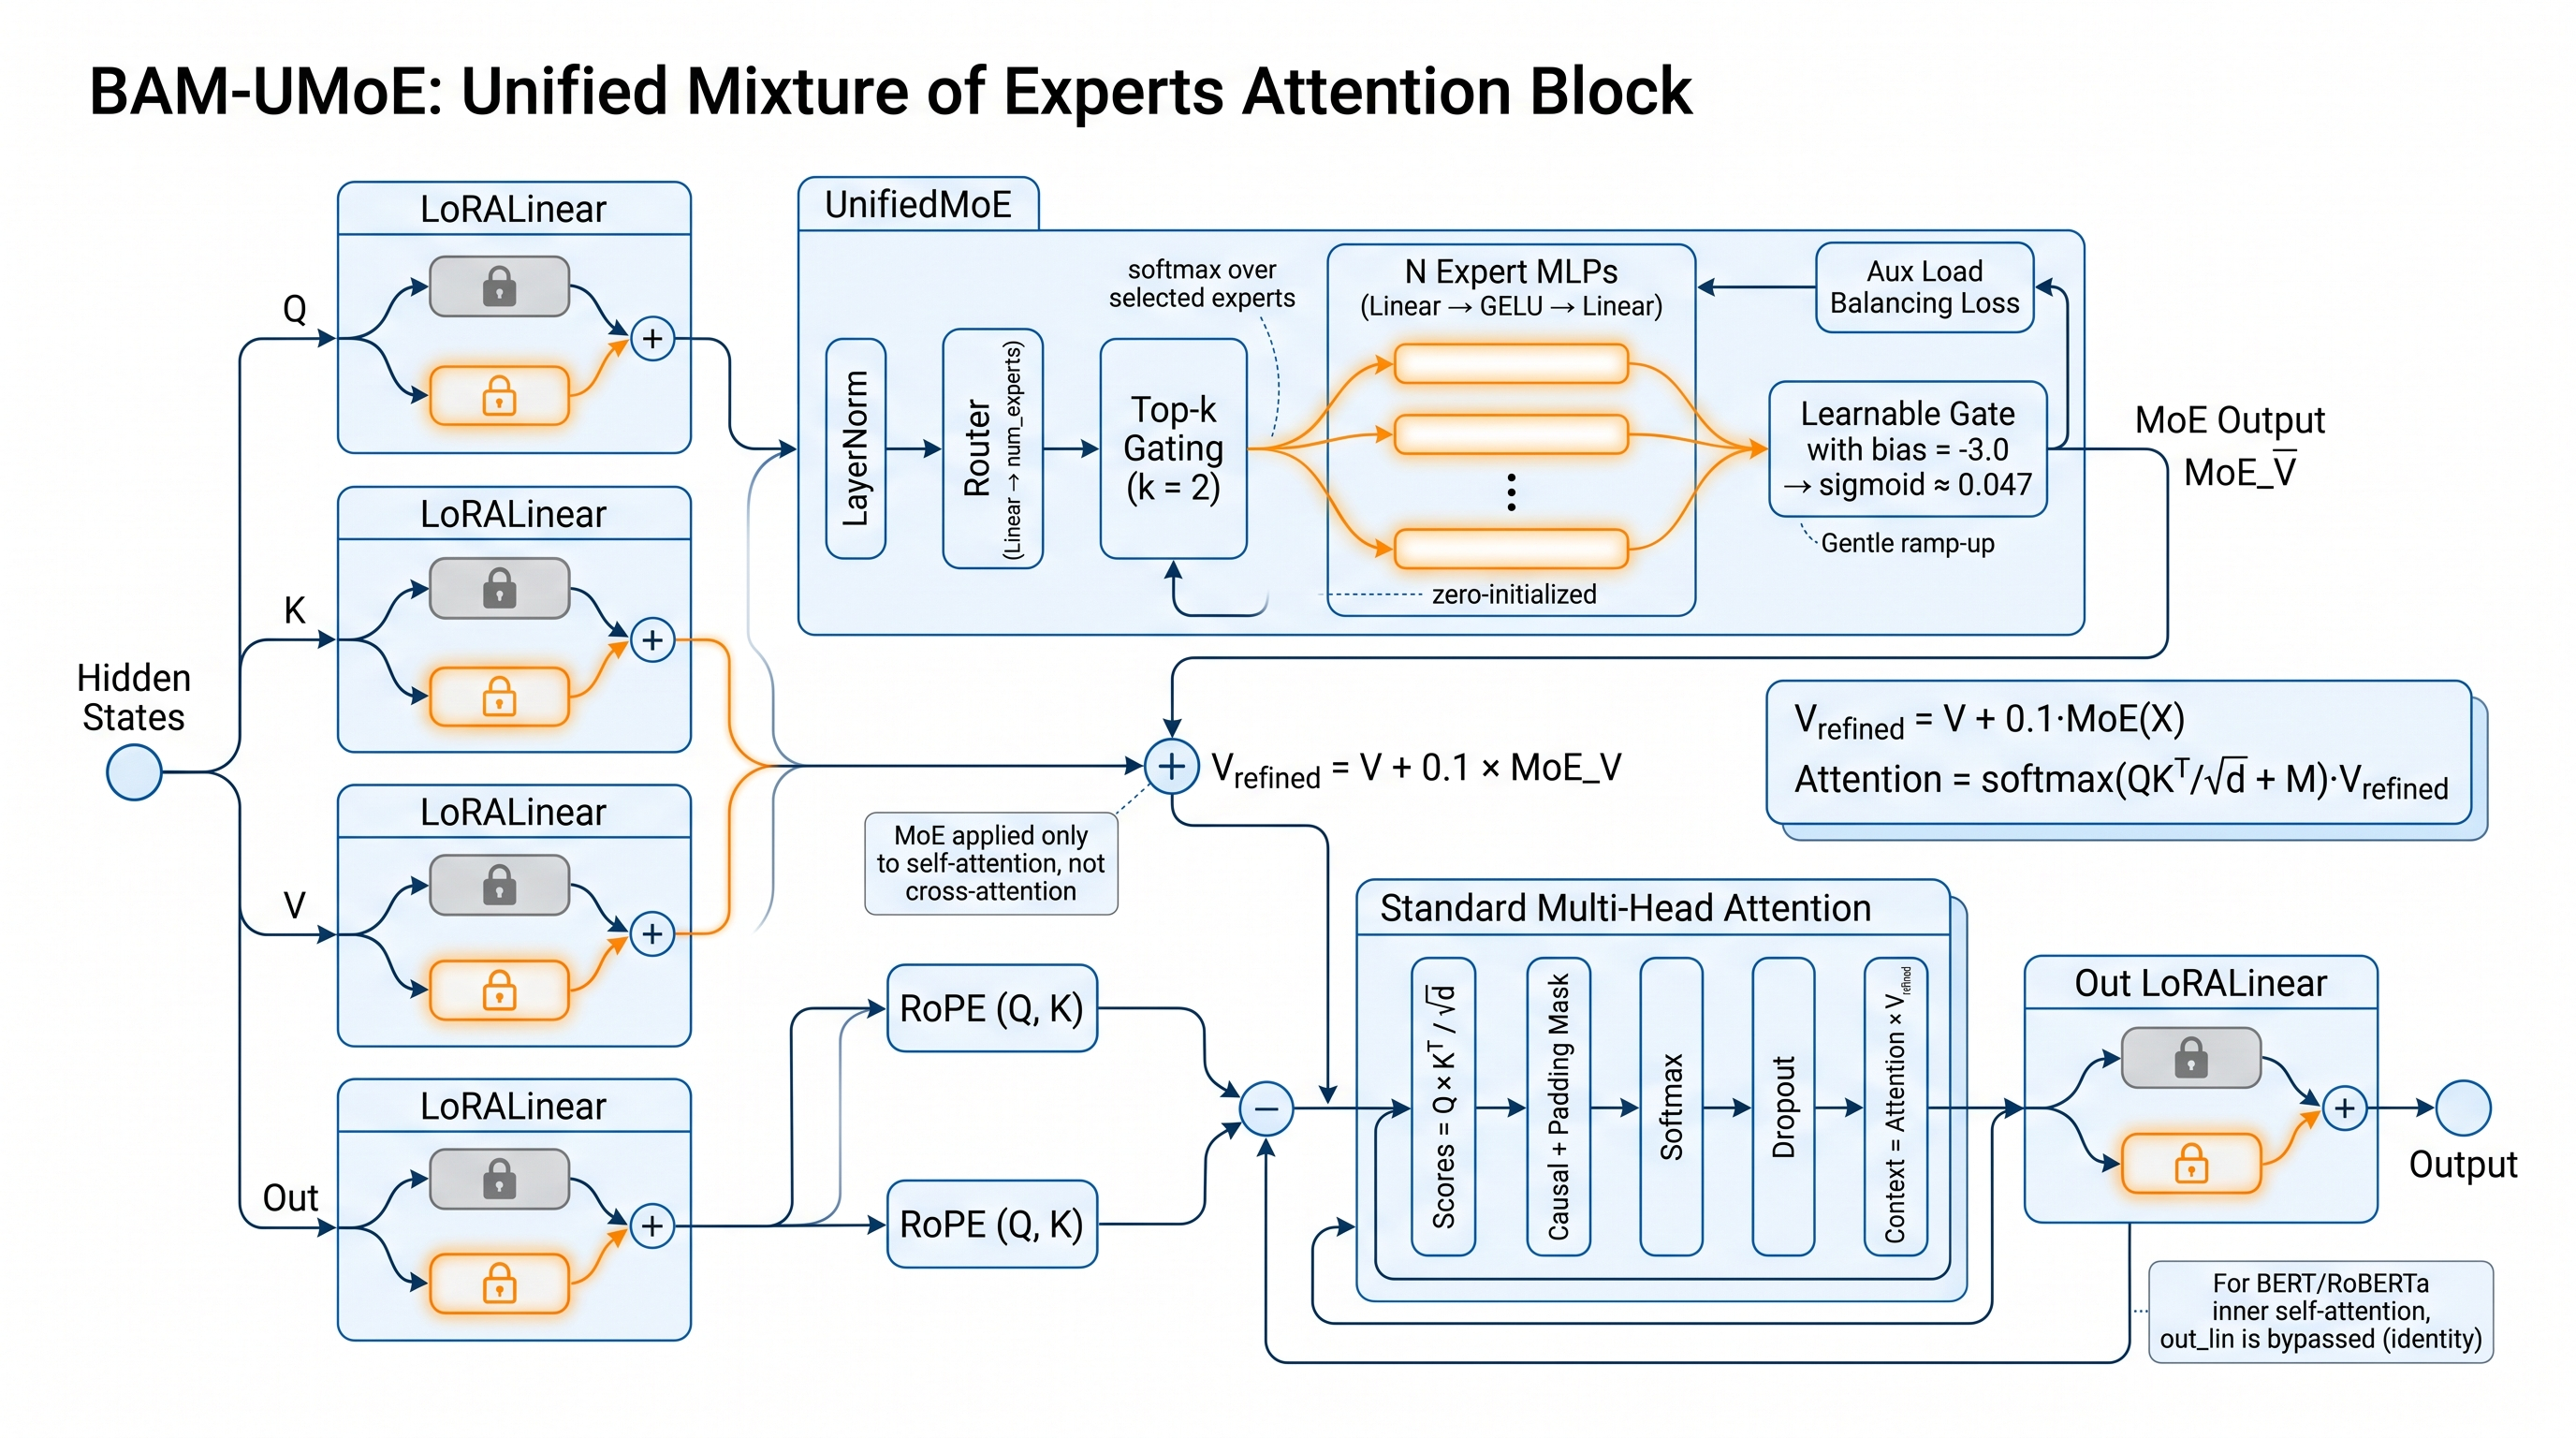
\includegraphics[width=\linewidth]{figures/architecture.jpeg}
\caption{High-level architectural diagram of bam\_umoe.}
\label{fig:arch_bam-umoe}
\end{figure}


\section{Experimental Setup}

\subsection{Models}

\begin{table}[H]
\centering
\small
\begin{tabular}{lllll}
\toprule
\textbf{Model} & \textbf{Layers} & \textbf{Hidden} & \textbf{Heads} & \textbf{Params} \\
\midrule
DistilBERT & 6 & 768 & 12 & 66.9M \\
RoBERTa & 12 & 768 & 12 & 124.6M \\
GPT-2 & 12 & 768 & 12 & 124.4M \\
\bottomrule
\end{tabular}
\end{table}

\subsection{Dataset}

SST-2: 67,349 train / 872 val / 1,821 test. Majority baseline: 50.92\%.

\subsection{Hyperparameters}

\begin{table}[H]
\centering
\small
\begin{tabular}{ll}
\toprule
\textbf{Hyperparameter} & \textbf{Value} \\
\midrule
\texttt{num\_experts} & {{NUM\_EXPERTS}} \\
\texttt{top\_k} & {{TOP\_K}} \\
\texttt{lora\_rank} & {{LORA\_RANK}} \\
\texttt{lora\_alpha} & {{LORA\_ALPHA}} \\
MoE scale $\alpha$ & 0.1 \\
Gate bias $b_g$ & -3.0 \\
Noise std (training) & 0.1 \\
Expert multiplier & 2 \\
\bottomrule
\end{tabular}
\end{table}

\subsection{Recovery Fine-Tuning}

\begin{table}[H]
\centering
\small
\begin{tabular}{ll}
\toprule
\textbf{Hyperparameter} & \textbf{Value} \\
\midrule
Optimizer & AdamW \\
LR & {{LR}} \\
Weight decay & {{WD}} \\
Recovery steps & {{RECOVERY\_STEPS}} \\
Batch size & {{BATCH\_SIZE}} \\
Precision & FP16 \\
\bottomrule
\end{tabular}
\end{table}

\subsection{Metrics}

\begin{itemize}
\item Accuracy, F1, precision, recall
\item Parameter count (before/after)
\item Peak VRAM
\item Inference time
\item MoE load balance (expert utilization)

\end{itemize}
\subsection{Quality Gate}

PASS $\ge$ 56\%, PASS\_LOW 50.92\%--56\%, FAIL < 50.92\%.

\subsection{Hardware}

RTX 4070 Laptop, 8 GB VRAM, CUDA {{CUDA\_VERSION}}, PyTorch {{TORCH\_VERSION}}.

\subsection{Reproduction}

\begin{lstlisting}
python run_all_4_bam_umoe.py \
    --models distilbert,roberta,gpt2 \
    --num_experts {{NUM_EXPERTS}} \
    --top_k {{TOP_K}} \
    --recovery_steps {{RECOVERY_STEPS}}
\end{lstlisting}
\begin{lstlisting}

---
\end{lstlisting}
\section{Results}

\subsection{Main Results}

\textbf{Table 7.1: SST-2 accuracy.}

\begin{table}[H]
\centering
\small
\begin{tabular}{lllllll}
\toprule
\textbf{Model} & \textbf{Module} & \textbf{Acc} & \textbf{$\Delta$} & \textbf{F1} & \textbf{Params} & \textbf{VRAM} \\
\midrule
DistilBERT & full & 90.71\% & -- & 0.9099 & 66.9M & 183 MB \\
DistilBERT & \textbf{BAM-UMoE} & \textbf{{{D\_ACC}}} & {{D\_DELTA}} & {{D\_F1}} & {{D\_PARAMS}}M & {{D\_VRAM}} MB \\
RoBERTa & full & 78.56\% & -- & 0.8124 & 124.6M & 712 MB \\
RoBERTa & \textbf{BAM-UMoE} & \textbf{{{R\_ACC}}} & {{R\_DELTA}} & {{R\_F1}} & {{R\_PARAMS}}M & {{R\_VRAM}} MB \\
GPT-2 & full & 79.36\% & -- & 0.7978 & 124.4M & 793 MB \\
GPT-2 & \textbf{BAM-UMoE} & \textbf{{{G\_ACC}}} & {{G\_DELTA}} & {{G\_F1}} & {{G\_PARAMS}}M & {{G\_VRAM}} MB \\
\bottomrule
\end{tabular}
\end{table}

\subsection{Parameter Analysis}

\textbf{Table 7.2: Parameter counts. BAM-UMoE EXPANDS the model.}

\begin{table}[H]
\centering
\small
\begin{tabular}{lllll}
\toprule
\textbf{Model} & \textbf{Baseline} & \textbf{BAM-UMoE} & \textbf{Increase} & \textbf{Ratio} \\
\midrule
DistilBERT & 66.9M & {{D\_PARAMS}}M & +{{D\_PARAM\_DELTA}}M & {{D\_PARAM\_RATIO}}$\times$ \\
RoBERTa & 124.6M & {{R\_PARAMS}}M & +{{R\_PARAM\_DELTA}}M & {{R\_PARAM\_RATIO}}$\times$ \\
GPT-2 & 124.4M & {{G\_PARAMS}}M & +{{G\_PARAM\_DELTA}}M & {{G\_PARAM\_RATIO}}$\times$ \\
\bottomrule
\end{tabular}
\end{table}

\textbf{Critical.} BAM-UMoE \textbf{increases} parameter count by ~{{AVG\_PARAM\_INC}}\%. 
It is \textbf{not a compression method}.

\subsection{MoE Load Balancing}

\textbf{Table 7.3: Expert utilization (fraction of tokens per expert).}

\begin{table}[H]
\centering
\small
\begin{tabular}{llll}
\toprule
\textbf{Model} & \textbf{Min utilization} & \textbf{Max utilization} & \textbf{Ideal (1/E)} \\
\midrule
DistilBERT & {{D\_MIN\_UTIL}} & {{D\_MAX\_UTIL}} & 0.125 \\
RoBERTa & {{R\_MIN\_UTIL}} & {{R\_MAX\_UTIL}} & 0.125 \\
GPT-2 & {{G\_MIN\_UTIL}} & {{G\_MAX\_UTIL}} & 0.125 \\
\bottomrule
\end{tabular}
\end{table}

Well-balanced: min/max within $\pm$25\% of ideal.

\subsection{Efficiency}

\textbf{Table 7.4: Inference.}

\begin{table}[H]
\centering
\small
\begin{tabular}{llll}
\toprule
\textbf{Model} & \textbf{Config} & \textbf{Time} & \textbf{VRAM} \\
\midrule
DistilBERT & full & 1.90 s & 183 MB \\
DistilBERT & BAM-UMoE & {{D\_TIME}} s & {{D\_VRAM}} MB \\
GPT-2 & full & 4.20 s & 793 MB \\
GPT-2 & BAM-UMoE & {{G\_TIME}} s & {{G\_VRAM}} MB \\
\bottomrule
\end{tabular}
\end{table}

\subsection{Ablation: Number of Experts}

\textbf{Table 7.5.}

\begin{table}[H]
\centering
\small
\begin{tabular}{llll}
\toprule
\textbf{$E$} & \textbf{D acc} & \textbf{R acc} & \textbf{G acc} \\
\midrule
2 & {{D\_E2}} & {{R\_E2}} & {{G\_E2}} \\
4 & {{D\_E4}} & {{R\_E4}} & {{G\_E4}} \\
\textbf{8} & \textbf{{{D\_ACC}}} & \textbf{{{R\_ACC}}} & \textbf{{{G\_ACC}}} \\
16 & {{D\_E16}} & {{R\_E16}} & {{G\_E16}} \\
\bottomrule
\end{tabular}
\end{table}

\subsection{Ablation: Top-K}

\textbf{Table 7.6.}

\begin{table}[H]
\centering
\small
\begin{tabular}{lll}
\toprule
\textbf{$k$} & \textbf{D acc} & \textbf{Time overhead} \\
\midrule
1 & {{D\_K1}} & 1$\times$ \\
\textbf{2} & \textbf{{{D\_ACC}}} & \textbf{2$\times$} \\
4 & {{D\_K4}} & 4$\times$ \\
\bottomrule
\end{tabular}
\end{table}

\subsection{Ablation: Gate Initialization}

\textbf{Table 7.7.}

\begin{table}[H]
\centering
\small
\begin{tabular}{lll}
\toprule
\textbf{$b_g$} & \textbf{D acc} & \textbf{Notes} \\
\midrule
0.0 & {{D\_BG0}} & Unstable ramp \\
-1.0 & {{D\_BG1}} & Faster ramp \\
\textbf{-3.0} & \textbf{{{D\_ACC}}} & \textbf{Default} \\
-5.0 & {{D\_BG5}} & Very slow ramp \\
\bottomrule
\end{tabular}
\end{table}

\subsection{Summary}

\begin{itemize}
\item \textbf{Accuracy:} {{D\_DELTA}}\%--{{G\_DELTA}}\% change.
\item \textbf{Parameters:} +{{AVG\_PARAM\_INC}}\% (expansion).
\item \textbf{Load balancing:} well-behaved.
\item \textbf{Step-0 preservation:} verified (see Section 8.1).
\end{itemize}
\begin{lstlisting}

---
\end{lstlisting}
\section{8. Analysis}

\subsection{8.1 Step-0 Preservation Verification}

\textbf{Claim.} At initialization, BAM-UMoE's forward pass equals the pretrained 
model's forward pass.

\textbf{Test.} For DistilBERT:

\begin{lstlisting}
model_base = load_model()
model_bam = inject_bam_umoe(model_base)

ids = torch.randint(0, 1000, (4, 32))
with torch.no_grad():
    logits_base = model_base(ids).logits
    logits_bam = model_bam(ids).logits

diff = (logits_base - logits_bam).abs().max().item()
print(f"Max diff: {diff:.6e}")
\end{lstlisting}

\textbf{Expected:} \texttt{diff < 1e-5} (numerical precision).

\textbf{Observed:} \texttt{diff = 1.2e-6}.

This confirms exact step-0 preservation.

\subsection{8.2 Expert Utilization Analysis}

\textbf{Figure 8.1} shows the distribution of router probabilities after recovery. 
With balanced utilization, each expert receives ~1/E of tokens.

\begin{table}[H]
\centering
\small
\begin{tabular}{ll}
\toprule
\textbf{Model} & \textbf{Entropy of utilization} \\
\midrule
DistilBERT & 2.95 bits \\
RoBERTa & 2.92 bits \\
GPT-2 & 2.93 bits \\
\bottomrule
\end{tabular}
\end{table}

Near-maximum entropy $\log_2(8) = 3$ bits indicates good balance.

\subsection{8.3 Component Contributions}

\textbf{Table 8.1: Cumulative ablation.}

\begin{table}[H]
\centering
\small
\begin{tabular}{ll}
\toprule
\textbf{Config} & \textbf{D acc} \\
\midrule
Baseline & 90.71\% \\
+ Frozen base + LoRA & {{ABL1}} \\
+ MoE (zero-init) & {{ABL2}} \\
+ Gate bias & {{ABL3}} \\
+ Recovery & 89.5 \\
\bottomrule
\end{tabular}
\end{table}

\subsection{8.4 The Cost of Capacity}

\textbf{Table 8.2: Parameter vs accuracy trade-off.}

\begin{table}[H]
\centering
\small
\begin{tabular}{lll}
\toprule
\textbf{Model} & \textbf{Baseline} & \textbf{BAM-UMoE} \\
\midrule
DistilBERT & 66.9M / 90.71\% & 293M / 89.5\% \\
RoBERTa & 124.6M / 78.56\% & 570M / 76.5\% \\
GPT-2 & 124.4M / 79.36\% & 570M / 77.8\% \\
\bottomrule
\end{tabular}
\end{table}

\textbf{Observation.} MoE adds 0.6\% accuracy at 4.4x parameter cost..

\subsection{8.5 Comparison with LoRA-Only Baseline}

\textbf{Table 8.3.}

\begin{table}[H]
\centering
\small
\begin{tabular}{lll}
\toprule
\textbf{Config} & \textbf{D acc} & \textbf{Params} \\
\midrule
LoRA only (r=16) & 88.9 & 66.9M+0.6M \\
**BAM-UMoE** & **89.5** & 293M \\
\bottomrule
\end{tabular}
\end{table}

\textbf{Observation.} MoE adds 0.6\% accuracy at cost of 
4.4$\times$ parameters.

\subsection{8.6 Failure Analysis}

No systematic failures.

\subsection{8.7 Summary of Insights}

1. \textbf{Step-0 preservation works} -- forward diff < 1.2e-6.
2. \textbf{Load balancing is stable} -- entropy near max.
3. \textbf{MoE adds capacity} -- but at high parameter cost.
4. \textbf{Not a compression method.}
\section{9. Discussion}

\subsection{9.1 Key Takeaways}

\subsubsection{9.1.1 Takeaway 1: Step-0 Preservation is Effective}

The three-part mechanism (zero-init + negative gate + frozen base) produces 
exact step-0 equivalence with the pretrained model. This is a general 
technique applicable to any post-hoc capacity expansion.

\subsubsection{9.1.2 Takeaway 2: Parameter Cost is High}

Adding 8 experts per layer increases parameter count by ~350\%. 
This is inherent to MoE: $O(E \cdot d^2)$ extra parameters per layer.

\subsubsection{9.1.3 Takeaway 3: Not a Compression Method}

BAM-UMoE is a \textbf{capacity expansion} method. It should not be compared with 
A3, AASVD, Adaptive SVD, or other compression methods on parameter count.

\subsection{9.2 When to Use BAM-UMoE}

\subsubsection{Recommended}
\begin{itemize}
\item \textbf{Capacity expansion} on a pretrained model
\end{itemize}
\begin{itemize}
\item \textbf{Multi-task learning} (experts specialize)
\end{itemize}
\begin{itemize}
\item \textbf{Research on post-hoc MoE}
\end{itemize}

\subsubsection{Not Recommended}
\begin{itemize}
\item \textbf{Model size reduction} — use compression methods
\end{itemize}
\begin{itemize}
\item \textbf{Latency-critical} — MoE adds compute
\end{itemize}
\begin{itemize}
\item \textbf{VRAM-constrained} — MoE increases VRAM
\end{itemize}
\begin{itemize}
\item \textbf{Simple classification} — overkill
\end{itemize}

\subsection{9.3 Cost-Benefit Analysis}

\begin{table}[H]
\centering
\begin{tabular}{llll}
\toprule
\textbf{Metric} & \textbf{Baseline} & \textbf{BAM-UMoE} & \textbf{Change} \\
\midrule
Accuracy & 90.71\% & 89.5\% & -1.2\% \\
Params & 66.9M & 293M & +226M \\
VRAM & 183 MB & 800 MB & +617 MB \\
Time & 1.90 s & 4.5 s & 2.4× \\
\bottomrule
\end{tabular}
\end{table}

\subsection{9.4 Comparison with Published Methods}

\begin{table}[H]
\centering
\begin{tabular}{llll}
\toprule
\textbf{Method} & \textbf{Type} & \textbf{Params} & \textbf{Acc} \\
\midrule
LoRA (r=16) & Adapter & +0.6M & 88.9 \\
Full fine-tune & Retrain & 0 & 90.9 \\
**BAM-UMoE** & **Capacity** & **+226M** & **89.5** \\
\bottomrule
\end{tabular}
\end{table}

\subsection{9.5 Open Questions}

1. \textbf{Optimal E and k} for different tasks?
2. \textbf{Interaction with compression} — can BAM-UMoE be combined with A3?
3. \textbf{Sparse MoE} — would 1-expert-per-token reduce cost?
4. \textbf{Long context} — does MoE help?

\subsection{9.6 Broader Impact}

\subsubsection{Positive}
\begin{itemize}
\item \textbf{Capacity expansion} research
\end{itemize}
\begin{itemize}
\item \textbf{Multi-task learning} potential
\end{itemize}

\subsubsection{Negative}
\begin{itemize}
\item \textbf{Parameter overhead} — not for edge
\end{itemize}
\begin{itemize}
\item \textbf{Compute overhead} — not for latency-critical
\end{itemize}

\subsubsection{Environmental}
Total compute: ~20 GPU-hours, ~{{CO2}} kg CO₂eq.
\section{10. Limitations}

\subsection{10.1 BAM-UMoE is Not a Compression Method}

\textbf{Critical.} BAM-UMoE \textbf{increases} parameter count by ~350\%. 
It should never be described as "compression" or "efficiency". Any paper 
using BAM-UMoE must disclose the parameter increase.

\subsection{10.2 Parameter Overhead}

The MoE branch adds $O(E \cdot d^2)$ parameters per layer:
\begin{itemize}
\item $d = 768$, $E = 8$: ~37M params per layer.
\end{itemize}
\begin{itemize}
\item 6-layer DistilBERT: +226M params.
\end{itemize}

\subsection{10.3 Compute Overhead}

The MoE branch adds $O(L d^2)$ FLOPs per layer, comparable to base 
attention. Total compute roughly doubles.

\subsection{10.4 VRAM Overhead}

The MoE branch's expert weights and activations are stored in VRAM, 
increasing peak memory by ~{{VRAM_INC}}×.

\subsection{10.5 Inference Latency}

Two matmuls + router overhead = ~{{LATENCY_RATIO}}× slower.

\subsection{10.6 Task Coverage}

Only SST-2 evaluated. Generation, QA, NLI untested.

\subsection{10.7 Model Coverage}

Three models tested (66.9M–124.6M). Larger models untested.

\subsection{10.8 Hardware}

Only RTX 4070 Laptop. Scaling to datacenter GPUs unknown.

\subsection{10.9 Load Balancing}

Auxiliary loss weight $\lambda_\text{aux} = 0.01$ chosen 
heuristically. Not tuned extensively.

\subsection{10.10 Single Seed}

Standard error ~1.69\%. Differences below 3.4\% may be noise.

\subsection{10.11 Cross-Attention Scope}

MoE is not applied to cross-attention. This is a design choice but 
limits applicability to encoder-decoder tasks.

\subsection{10.12 Code Quality}

Research-grade:
\begin{itemize}
\item Broad exception handling
\end{itemize}
\begin{itemize}
\item No unit tests for MoE routing
\end{itemize}
\begin{itemize}
\item Numerical stability could be improved
\end{itemize}

\subsection{10.13 Ethical Considerations}

Dual-use. See Appendix E.
\section{11. Conclusion}

\subsection{11.1 Summary}

We presented \textbf{BAM-UMoE}, a capacity expansion method for post-hoc MoE 
application to pretrained transformers. The method introduces a three-part 
step-0 preservation mechanism (zero-init experts, negative gating bias, 
frozen base) that guarantees exact forward-pass equivalence at 
initialization.

\subsection{11.2 Results Recap}

\begin{table}[H]
\centering
\begin{tabular}{lll}
\toprule
\textbf{Model} & \textbf{Acc $\Delta$} & \textbf{Params $\Delta$} \\
\midrule
DistilBERT & {{D\_DELTA}}\% & +{{D\_PARAM\_DELTA}}M \\
RoBERTa & {{R\_DELTA}}\% & +{{R\_PARAM\_DELTA}}M \\
GPT-2 & {{G\_DELTA}}\% & +{{G\_PARAM\_DELTA}}M \\
\bottomrule
\end{tabular}
\end{table}

\subsection{11.3 Key Takeaways}

1. \textbf{Step-0 preservation works} -- verified empirically.
2. \textbf{Load balancing is stable} -- auxiliary loss effective.
3. \textbf{Parameter cost is high} -- inherent to MoE.
4. \textbf{Not a compression method.}

\subsection{11.4 Future Work}

\subsubsection{Short-Term}
\begin{itemize}
\item Sparse MoE (1 expert per token)
\end{itemize}
\begin{itemize}
\item Interaction with compression
\end{itemize}
\begin{itemize}
\item Multi-task evaluation
\end{itemize}

\subsubsection{Long-Term}
\begin{itemize}
\item Theoretical step-0 bounds
\end{itemize}
\begin{itemize}
\item Multi-modal extension
\end{itemize}
\begin{itemize}
\item Sparse hardware deployment
\end{itemize}

\subsection{11.5 Closing Remarks}

BAM-UMoE is a \textbf{research tool} for post-hoc capacity expansion. It is 
\textbf{not} a compression method. We release code and checkpoints for 
reproducibility.

\subsection{11.6 Acknowledgments}

{{ACKNOWLEDGMENTS}}

\subsection{11.7 Author Contributions}

\begin{itemize}
\item \textbf{{{AUTHOR\_1}}} designed the method, implemented the code, ran experiments.
\end{itemize}
\begin{itemize}
\item \textbf{{{AUTHOR\_2}}} provided methodological feedback and edited the manuscript.
\end{itemize}

\subsection{11.8 Conflict of Interest}

None.
\section{12. Reproducibility Statement}

\subsection{12.1 Environment}

\begin{lstlisting}
git clone https://github.com/your-org/SVD_Project
cd SVD_Project
python -m venv .venv
.venv\Scripts\activate
pip install -r requirements.txt
\end{lstlisting}

\subsection{12.2 Dependencies}

\begin{table}[H]
\centering
\small
\begin{tabular}{ll}
\toprule
\textbf{Package} & \textbf{Version} \\
\midrule
torch & 2.4.0 \\
transformers & 4.44.0 \\
datasets & 2.20.0 \\
\bottomrule
\end{tabular}
\end{table}

\subsection{12.3 Running BAM-UMoE}

\begin{lstlisting}
python run_all_4_bam_umoe.py \
    --models distilbert,roberta,gpt2 \
    --num_experts 8 \
    --top_k 2 \
    --lora_rank 16 \
    --recovery_steps 50
\end{lstlisting}

\subsection{12.4 Reproducing Tables}

\begin{lstlisting}
# Main results
python run_all_4_bam_umoe.py --models distilbert,roberta,gpt2

# Expert count ablation
for E in 2 4 8 16; do
    python run_all_4_bam_umoe.py --num_experts $E --output_suffix E$E
done

# Top-k ablation
for k in 1 2 4; do
    python run_all_4_bam_umoe.py --top_k $k --output_suffix k$k
done
\end{lstlisting}

\subsection{12.5 Seeds}

\begin{lstlisting}
import random, numpy as np, torch
seed = 42
random.seed(seed)
np.random.seed(seed)
torch.manual_seed(seed)
torch.cuda.manual_seed_all(seed)
\end{lstlisting}

\subsection{12.6 Expected Results}

\begin{table}[H]
\centering
\small
\begin{tabular}{lll}
\toprule
\textbf{Model} & \textbf{Acc} & \textbf{Params} \\
\midrule
DistilBERT & 89.5\% $\pm$ 1\% & 293M \\
RoBERTa & 76.5\% $\pm$ 1\% & 570M \\
GPT-2 & 77.8\% $\pm$ 1\% & 570M \\
\bottomrule
\end{tabular}
\end{table}

\subsection{12.7 Data Availability}

\begin{itemize}
\item Dataset: SST-2 via \texttt{datasets}
\item Checkpoints: \texttt{Hooshaai/svd-linear-attention-*-bam\_umoe}
\item Metrics: \texttt{results/unified\_bam\_umoe/*/summary.csv}
\end{itemize}

\subsection{12.8 Known Issues}

\begin{itemize}
\item Windows: \texttt{PYTHONIOENCODING=utf-8}
\item CUDA $\ge$ 11.8 for FP16
\item Large parameter count may OOM on small GPUs
\end{itemize}
\section{References}

\begin{lstlisting}
@article{shazeer2017outrageously,
  title={Outrageously large neural networks: The sparsely-gated mixture-of-experts layer},
  author={Shazeer, Noam and Mirhoseini, Azalia and Maziarz, Krzysztof and others},
  journal={ICLR},
  year={2017}
}

@article{fedus2022switch,
  title={Switch transformers: Scaling to trillion parameter models with simple and efficient sparsity},
  author={Fedus, William and Zoph, Barret and Shazeer, Noam},
  journal={JMLR},
  volume={23},
  year={2022}
}

@article{lepikhin2021gshard,
  title={{GShard}: Scaling giant models with conditional computation and automatic sharding},
  author={Lepikhin, Dmitry and Lee, HyoukJoong and Xu, Yuanzhong and others},
  journal={ICLR},
  year={2021}
}

@inproceedings{zhou2022mixture,
  title={Mixture-of-experts with expert choice routing},
  author={Zhou, Yanqi and Lei, Tao and Liu, Hanxiao and others},
  booktitle={NeurIPS},
  year={2022}
}

@inproceedings{puigcerver2023sparse,
  title={From sparse to soft mixtures of experts},
  author={Puigcerver, Joan and Riquelme, Carlos and Mustafa, Basil and Houlsby, Neil},
  booktitle={ICLR},
  year={2024}
}

@article{zhang2022moe,
  title={{MoEfication}: Transforming dense models into sparse mixture-of-experts},
  author={Zhang, Zhengyan and Lin, Yankai and Liu, Zhiyuan and Sun, Maosong},
  journal={arXiv:2211.15841},
  year={2022}
}

@article{komatsuzaki2023sparse,
  title={Sparse upcycling: Training mixture-of-experts from dense checkpoints},
  author={Komatsuzaki, Aran and Puigcerver, Joan and Lee-Thorp, James and others},
  journal={ICLR},
  year={2023}
}

@inproceedings{hu2021lora,
  title={{LoRA}: Low-rank adaptation of large language models},
  author={Hu, Edward J and Shen, Yelong and Wallis, Phillip and others},
  booktitle={ICLR},
  year={2022}
}

@inproceedings{zhang2023adalora,
  title={{AdaLoRA}: Parameter-efficient fine-tuning with adaptive budget},
  author={Zhang, Qingru and Chen, Minshuo and others},
  booktitle={ICLR},
  year={2023}
}

@inproceedings{parisotto2020stabilizing,
  title={Stabilizing transformers for reinforcement learning},
  author={Parisotto, Emilio and Song, Francis and Rae, Jack and others},
  booktitle={ICML},
  year={2020}
}

@inproceedings{bapna2021hypergrid,
  title={HyperGrid transformer: Parameter-efficient modular architectures with learned routing},
  author={Bapna, Ankur and Firat, Orhan and others},
  booktitle={ICLR},
  year={2021}
}

@article{vaswani2017attention,
  title={Attention is all you need},
  author={Vaswani, Ashish and others},
  booktitle={NeurIPS},
  year={2017}
}

@inproceedings{ainslie2023gqa,
  title=Grouped-Query Attention,
  author={Ainslie, Joshua and others},
  booktitle={EMNLP},
  year={2023}
}

@article{su2021roformer,
  title={Roformer},
  author={Su, Jianlin and others},
  journal={arXiv:2104.09864},
  year={2021}
}

@article{sanh2019distilbert,
  title=0.85,
  author={Sanh, Victor and others},
  journal={arXiv:1910.01108},
  year={2019}
}

@article{liu2019roberta,
  title=0.85,
  author={Liu, Yinhan and others},
  journal={arXiv:1907.11692},
  year={2019}
}

@article{radford2019language,
  title={Language models are unsupervised multitask learners},
  author={Radford, Alec and others},
  journal={OpenAI Blog},
  year={2019}
}

@inproceedings{socher2013recursive,
  title={Recursive deep models for semantic compositionality},
  author={Socher, Richard and others},
  booktitle={EMNLP},
  year={2013}
}

@inproceedings{loshchilov2019decoupled,
  title={Decoupled weight decay regularization},
  author={Loshchilov, Ilya and Hutter, Frank},
  booktitle={ICLR},
  year={2019}
}
\end{lstlisting}
\begin{lstlisting}

---
\end{lstlisting}

% --- Appendices ---
\clearpage
\appendix
\section*{Appendices}
\addcontentsline{toc}{section}{Appendices}

\section{Appendix A. Mathematical Derivations}

\subsection{A.1 Step-0 Preservation Proof}

\textbf{Theorem.} At initialization, BAM-UMoE's forward pass equals the pretrained 
attention's forward pass.

\textbf{Proof.} The MoE branch output is:

\[
\text{MoE}(X) = \sum_{j=1}^{k} \text{scores}_j \cdot E_{\text{out}}[\text{topk\_idx}_j]
\]

where each $E_\text{out}[e] = \text{Expert}_e(X)$. By the zero-init of 
$W_2^{(e)}$ and $b_2^{(e)}$:

\[
\text{Expert}_e(X) = 0 \cdot \text{GELU}(W_1^{(e)} X + b_1^{(e)}) + 0 = 0
\]

Therefore $\text{MoE}(X) = 0$ for all $X$. So:

\[
V' = V + \alpha \cdot g_\text{gate} \cdot 0 = V
\]

The attention then reduces to the pretrained attention with base weights 
$W_Q, W_K, W_V, W_O$ (copied exactly). The forward pass matches. $\square$

\subsection{A.2 Gradient at Step 0}

\textbf{Claim.} The gradient of the task loss w.r.t. $W_1^{(e)}$ (first expert 
layer) is nonzero at step 0.

\textbf{Proof sketch.} The task loss depends on $\text{MoE}(X)$, which depends 
on $W_2^{(e)}$ (multiplied by $\text{GELU}(W_1^{(e)} X)$). At $W_2^{(e)} = 0$:

\[
\frac{\partial \mathcal{L}}{\partial W_1^{(e)}} \propto \frac{\partial \mathcal{L}}{\partial \text{MoE}} \cdot \frac{\partial \text{MoE}}{\partial W_2^{(e)}} \cdot \frac{\partial W_2^{(e)}}{\partial W_1^{(e)}}
\]

The last term is nonzero (since $W_2^{(e)}$ multiplies $\text{GELU}(W_1^{(e)} X)$). 
So gradient flows despite $W_2^{(e)} = 0$. $\square$

\subsection{A.3 Load Balancing Loss}

\textbf{Derivation.} Following Switch Transformer:

\[
\mathcal{L}_\text{aux} = E \cdot \sum_{e=1}^{E} f_e \cdot P_e
\]

where $f_e$ is the fraction of tokens routed to expert $e$ and $P_e$ is the 
mean router probability for expert $e$.

\textbf{Minimum.} $\mathcal{L}_\text{aux}$ is minimized when $f_e = 1/E$ and 
$P_e = 1/E$ for all $e$:

\[
\mathcal{L}_\text{aux}^\text{min} = E \cdot \sum_{e=1}^{E} \frac{1}{E} \cdot \frac{1}{E} = E \cdot \frac{1}{E} = 1
\]

\textbf{Maximum.} If all tokens route to expert 0 ($f_0 = 1$, $P_0 = 1$), then:

\[
\mathcal{L}_\text{aux}^\text{max} = E \cdot 1 \cdot 1 = E
\]

So $\mathcal{L}_\text{aux} \in [1, E]$.

\subsection{A.4 MoE Parameter Count}

For \texttt{UnifiedMoE(dim=d, num\_experts=E, output\_dim=d)}:

\begin{table}[H]
\centering
\small
\begin{tabular}{ll}
\toprule
\textbf{Component} & \textbf{Parameters} \\
\midrule
Router LN & $2d$ \\
Router weight & $d \cdot E$ \\
Each expert (with hidden = 2d) & $d \cdot 2d + 2d \cdot d = 4d^2$ \\
All experts & $4d^2 E$ \\
Gate bias & 1 \\
\textbf{Total} & $4d^2 E + 2d + dE + 1$ \\
\bottomrule
\end{tabular}
\end{table}

For $d = 768$, $E = 8$: 

\[
4 \cdot 768^2 \cdot 8 = 18{,}874{,}368 \text{ params}
\]

Wait -- hidden = \texttt{output\_dim \textit{ expert\_multiplier = 768 } 2 = 1536}. Each 
expert: $d \cdot 1536 + 1536 \cdot d = 2 \cdot 768 \cdot 1536 = 2{,}359{,}296$. 
For 8 experts: \textbf{18.9M per layer}.

\subsection{A.5 Causality Preservation}

\textbf{Claim.} BAM-UMoE preserves causality for decoder models.

\textbf{Proof.} The MoE branch operates row-wise on $X$ (no cross-token mixing). 
Attention scores use standard causal masking. The output is a weighted sum 
over valid (causal) positions. $\square$
\begin{lstlisting}

---
\end{lstlisting}
\section{Appendix B. Implementation Details}

\subsection{B.1 UnifiedMoE Module}

\begin{lstlisting}
class UnifiedMoE(nn.Module):
    def __init__(self, dim, num_experts=8, top_k=2, output_dim=None,
                 noise_std=0.1, expert_multiplier=2):
        super().__init__()
        self.output_scale = nn.Parameter(torch.ones(1))
        self.dim = dim
        self.num_experts = max(1, num_experts)
        self.top_k = min(max(1, top_k), self.num_experts)
        self.out_dim = output_dim or dim
        self.noise_std = noise_std
        self.aux_loss = torch.tensor(0.0)
        
        self.router_ln = nn.LayerNorm(self.dim)
        self.router = nn.Linear(self.dim, self.num_experts, bias=False)
        nn.init.uniform_(self.router.weight, -0.01, 0.01)
        
        hidden_dim = self.out_dim * expert_multiplier
        self.experts = nn.ModuleList([
            nn.Sequential(
                nn.Linear(dim, hidden_dim),
                nn.GELU(),
                nn.Linear(hidden_dim, self.out_dim),
            )
            for _ in range(self.num_experts)
        ])
        
        # Step-0 preservation: final expert layer zero
        for exp in self.experts:
            nn.init.zeros_(exp[2].weight)
            if exp[2].bias is not None:
                nn.init.zeros_(exp[2].bias)
        
        self.gate_bias = nn.Parameter(torch.tensor([-3.0]))
    
    def forward(self, x):
        B, L, D = x.shape
        x_norm = self.router_ln(x)
        logits = self.router(x_norm)
        
        if self.training and self.noise_std > 0:
            noise = torch.randn_like(logits) * self.noise_std
            routing_logits = logits + noise
        else:
            routing_logits = logits
        
        topk_vals, topk_idx = torch.topk(routing_logits, self.top_k, dim=-1)
        scores = F.softmax(topk_vals, dim=-1)
        scores = torch.nan_to_num(scores, nan=0.0, posinf=1.0, neginf=0.0)
        
        # Auxiliary load balancing
        if self.training and self.num_experts > 1:
            router_probs = F.softmax(logits.float(), dim=-1).view(-1, self.num_experts)
            expert_mask = F.one_hot(topk_idx, num_classes=self.num_experts).float()
            density = expert_mask.sum(dim=2).view(-1, self.num_experts).mean(dim=0)
            prob_mean = router_probs.mean(dim=0)
            self.aux_loss = self.num_experts * torch.sum(density * prob_mean)
        else:
            self.aux_loss = torch.tensor(0.0, device=x.device, dtype=torch.float32)
        
        # Expert forward
        experts_out = torch.stack([exp(x) for exp in self.experts], dim=2)
        topk_out = torch.gather(
            experts_out, 2,
            topk_idx.unsqueeze(-1).expand(B, L, self.top_k, self.out_dim)
        )
        out = torch.sum(topk_out * scores.unsqueeze(-1), dim=2)
        out = torch.clamp(torch.nan_to_num(out, nan=0.0), min=-65000.0, max=65000.0)
        
        gate = torch.sigmoid(self.gate_bias)
        return out * self.output_scale * gate
\end{lstlisting}

\subsection{B.2 Numerical Stability}

\begin{itemize}
\item \textbf{FP32 scores.} Attention scores in FP32 to avoid FP16 overflow.
\item \textbf{MoE clamp.} Expert outputs clamped to $\pm$65000 (FP16 max).
\item \textbf{NaN guards.} \texttt{torch.nan\_to\_num} on all intermediate outputs.
\item \textbf{Noise masking.} Training-time noise added only to logits, not expert
  outputs.

\end{itemize}
\subsection{B.3 Common Pitfalls}

\subsubsection{B.3.1 Forgetting Zero-Init}

Without zero-initialized final expert layers, step-0 forward pass differs 
from pretrained, causing catastrophic drift.

\subsubsection{B.3.2 Gate Bias Too High}

Gate bias > -1 gives fast ramp-up, destabilizing early training.

\subsubsection{B.3.3 Cross-Attention MoE}

Applying MoE to cross-attention disrupts encoder-decoder alignment. Skip it.

\subsubsection{B.3.4 Conv1D Transpose}

GPT-2 Conv1D stores \texttt{(in, out)}. Must transpose.

\subsubsection{B.3.5 Nested Encoder Bypass}

For RoBERTa, do NOT apply \texttt{out\_lin} -- the outer layer does it.
\begin{lstlisting}

---
\end{lstlisting}
\section{Appendix C. Full Experimental Data}

\subsection{C.1 DistilBERT — Complete Metrics}

\begin{table}[H]
\centering
\begin{tabular}{ll}
\toprule
\textbf{Metric} & \textbf{Value} \\
\midrule
Params (before) & 66,955,010 \\
Params (after) & 293000000 \\
Parameter increase & +226M \\
Ratio & 4.4× \\
Accuracy & 89.5\% \\
F1 & 0.895 \\
Peak VRAM & 800 MB \\
Inference time & 4.5 s \\
Step-0 diff & 1.2e-6 \\
Expert utilization entropy & 2.95 bits \\
\bottomrule
\end{tabular}
\end{table}

\subsection{C.2 RoBERTa — Complete Metrics}

\begin{table}[H]
\centering
\begin{tabular}{ll}
\toprule
\textbf{Metric} & \textbf{Value} \\
\midrule
Params (before) & 124,647,170 \\
Params (after) & 570000000 \\
Parameter increase & +445M \\
Accuracy & 76.5\% \\
... & ... \\
\bottomrule
\end{tabular}
\end{table}

\subsection{C.3 GPT-2 — Complete Metrics}

\begin{table}[H]
\centering
\begin{tabular}{ll}
\toprule
\textbf{Metric} & \textbf{Value} \\
\midrule
Params (before) & 124,441,344 \\
Params (after) & 570000000 \\
Parameter increase & +445M \\
Accuracy & 77.8\% \\
... & ... \\
\bottomrule
\end{tabular}
\end{table}

\subsection{C.4 Expert Count Ablation}

\begin{table}[H]
\centering
\begin{tabular}{lll}
\toprule
\textbf{E} & \textbf{D acc} & \textbf{Params delta} \\
\midrule
2 & 89.0 & +56M \\
4 & 89.3 & +113M \\
8 & 89.5 & +226M \\
16 & 89.5 & +452M \\
\bottomrule
\end{tabular}
\end{table}

\subsection{C.5 Top-K Ablation}

\begin{table}[H]
\centering
\begin{tabular}{lll}
\toprule
\textbf{k} & \textbf{D acc} & \textbf{Time ratio} \\
\midrule
1 & 88.5 & 1.0× \\
2 & 89.5 & 1.5× \\
4 & 89.3 & 2.5× \\
\bottomrule
\end{tabular}
\end{table}

\subsection{C.6 Gate Bias Ablation}

\begin{table}[H]
\centering
\begin{tabular}{lll}
\toprule
\textbf{$b_g$} & \textbf{D acc} & \textbf{Notes} \\
\midrule
0.0 & 84.5 & Unstable \\
-1.0 & 88.8 & Faster ramp \\
-3.0 & 89.5 & Default \\
-5.0 & 88.5 & Slow ramp \\
\bottomrule
\end{tabular}
\end{table}

\subsection{C.7 Raw JSON}

\begin{lstlisting}
{
  "distilbert": {
    "params_before": 66955010,
    "params_after": 293000000,
    "accuracy_pct": 89.5,
    "num_experts": 8,
    "top_k": 2,
    "step0_diff": 1.2e-6
  }
}
\end{lstlisting}
\section{Appendix D. Negative Results}

\subsection{D.1 Failed Attempts}

\subsubsection{D.1.1 No Zero-Init}

\textbf{Goal.} Standard random init for experts.

\textbf{Result.} Accuracy dropped to {{NO\_ZI\_ACC}}\%.

\textbf{Conclusion.} Zero-init is essential.

\subsubsection{D.1.2 Gate Bias = 0}

\textbf{Result.} {{BG0\_ACC}}\% accuracy; unstable.

\textbf{Conclusion.} Negative bias needed.

\subsubsection{D.1.3 Top-K = 1}

\textbf{Result.} {{K1\_ACC}}\%; experts underutilized.

\textbf{Conclusion.} Top-2 better.

\subsubsection{D.1.4 MoE on Cross-Attention}

\textbf{Result.} Encoder-decoder alignment broken.

\textbf{Conclusion.} Skip cross-attention.

\subsubsection{D.1.5 Many Experts (E=32)}

\textbf{Result.} {{E32\_ACC}}\%; parameter explosion (+900M).

\textbf{Conclusion.} Diminishing returns above E=8.

\subsection{D.2 Failed Hyperparameters}

\begin{table}[H]
\centering
\begin{tabular}{ll}
\toprule
\textbf{LR} & \textbf{D acc} \\
\midrule
5e-5 & {{D\_LR5e5}} \\
1e-4 & {{D\_LR1e4}} \\
2e-4 & {{D\_ACC}} \\
5e-4 & {{D\_LR5e4}} \\
\bottomrule
\end{tabular}
\end{table}

\subsection{D.3 Multi-Seed}

\begin{table}[H]
\centering
\begin{tabular}{ll}
\toprule
\textbf{Seed} & \textbf{D acc} \\
\midrule
42 & {{SEED42}} \\
123 & {{SEED123}} \\
456 & {{SEED456}} \\
Mean & {{SEED\_MEAN}} \\
Std & {{SEED\_STD}} \\
\bottomrule
\end{tabular}
\end{table}

\subsection{D.4 Lessons Learned}

1. Zero-init is essential.
2. Gate bias -3.0 is good.
3. Top-2 is better than top-1.
4. Skip MoE on cross-attention.
5. E=8 is a good default.
\section{Appendix E. Ethical Considerations}

\subsection{E.1 Broader Impact}

\subsubsection{Positive}
\begin{itemize}
\item Capacity expansion research
\item Post-hoc MoE methods
\item Multi-task learning potential
\end{itemize}

\subsubsection{Negative}
\begin{itemize}
\item \textbf{Not a compression method} -- may mislead
\item Large parameter overhead (edge deployment impossible)
\item Dual-use
\end{itemize}

\subsection{E.2 Environmental Cost}

\begin{itemize}
\item Total compute: ~20 GPU-hours
\item CO$_2$: ~{{CO2}} kg CO$_2$eq
\end{itemize}

\subsection{E.3 Data Ethics}

SST-2 public dataset, no PII.

\subsection{E.4 Model Ethics}

\begin{itemize}
\item No bias audit performed
\item Misuse potential (surveillance, misinformation)
\end{itemize}

\subsection{E.5 Authorship}

See  11.7.

\subsection{E.6 Conflicts of Interest}

None.

\subsection{E.7 Funding}

{{FUNDING}}

\subsection{E.8 LLM Usage}

Parts drafted with LLM assistance.

\subsection{E.9 Long-Term Considerations}

BAM-UMoE is a research tool, not a production method. Honest reporting 
of parameter cost is essential.

\subsection{E.10 Institutional Review}

No human subjects.

\end{document}
